\documentclass{article}

% NeurIPS 2026 style --- submission mode (anonymized)
\usepackage[final]{neurips_2026}

% Essential packages
\usepackage[utf8]{inputenc}
\usepackage[T1]{fontenc}
\usepackage{hyperref}
\hypersetup{hidelinks}
\usepackage{url}
\usepackage{booktabs}
\usepackage{amsfonts}
\usepackage{amssymb}
\usepackage{amsmath}
\usepackage{nicefrac}
\usepackage{microtype}
\usepackage{xcolor}
\usepackage{graphicx}
\usepackage{subcaption}
\usepackage{multirow}
\graphicspath{{figures/}}

\title{Why Transformers Fail at Counting and How to Fix It}

\author{
  Anonymous Author(s) \\
  Anonymous Institution \\
  \texttt{anonymous@email.com}
}

\begin{document}

\maketitle

\begin{abstract}
Large language models often fail at simple counting tasks, even when the items
to count are explicitly present in the prompt. We investigate whether this
failure occurs because transformers do not represent counts internally, or
because they cannot convert those representations into the correct output tokens.

Across three model families: Pythia, Qwen3, and Mistral, ranging from 0.4B to
14B parameters, we find strong evidence for the second explanation. Linear
probes recover the correct count from intermediate layers with near-perfect
accuracy ($R^2>0.99$), showing that the information is present. However, the
internal directions that encode counts are nearly orthogonal to the output-head
rows for digit tokens ($|\cos| \leq 0.032$). The model stores the count in a
form that the digit logits do not naturally read out.

We localize this failure with two interventions. Updating only the digit rows
of the output head (36,864 parameters) substantially improves constrained
next-token digit prediction (60.7--100.0\% across four tasks), but it does not
fix autoregressive generation. By contrast, a LoRA intervention on attention
Q/V weights (7.67M parameters) improves upstream routing and achieves
83.1\%\,$\pm$\,7.2\% in true greedy autoregressive generation. Logit-lens
measurements confirm the mechanism: the correct digit's vocabulary rank drops
from 55,980 to 1. The bottleneck generalizes
across character counting, addition, and list length, while remaining absent
from broader multi-step reasoning benchmarks (MMLU, GSM8K).

These results identify counting failure as a geometric readout bottleneck rather
than a failure of internal representation: the model knows the count but the
output pathway is geometrically misaligned with the tokens needed to express it.
\end{abstract}

% =============================================================================
\section{Introduction}
\label{sec:introduction}
% =============================================================================

\paragraph{Core claims.}
A transformer that fails to count could be failing at either of two stages: it
may never form an internal representation of the count, or it may form one and
be unable to convert it into the right output token. Distinguishing these
hypotheses requires measuring the internal representation directly (linear
probes), measuring how the output head reads it out (cosine alignment and
logit lens), and intervening on each stage in turn (targeted repairs). Under
this microscope, three nested claims emerge:

\begin{enumerate}
\item \textbf{Counts are linearly encoded but geometrically misaligned with
  digit rows.} Count-encoding directions are orthogonal to
  \texttt{lm\_head} digit rows ($|\cos| \leq 0.032$,
  indistinguishable from random). This is a structural property of the trained model.
\item \textbf{Repairing only the digit rows fixes constrained decoding, not
    generation.} The 9-row repair
  causally localizes the readout misalignment to digit rows \emph{for
  constrained digit decoding} (60.7--100.0\%). Under unconstrained autoregressive
  generation, the same repair achieves $0.0\%$, confirming the deployment
  bottleneck includes upstream routing beyond the output head.
\item \textbf{Correcting upstream routing restores generation.} LoRA Q/V rank-16 corrects
  upstream attention routing, achieving 83.1\%$\pm$7.2\% generation accuracy
  (5 seeds, multi-task; entity-only per-task: 97.0\%, 96.5\%, 94.5\%).
\end{enumerate}
Figure~\ref{fig:pipeline} summarizes the diagnosis and the three interventions.

\begin{figure}[t]
\centering
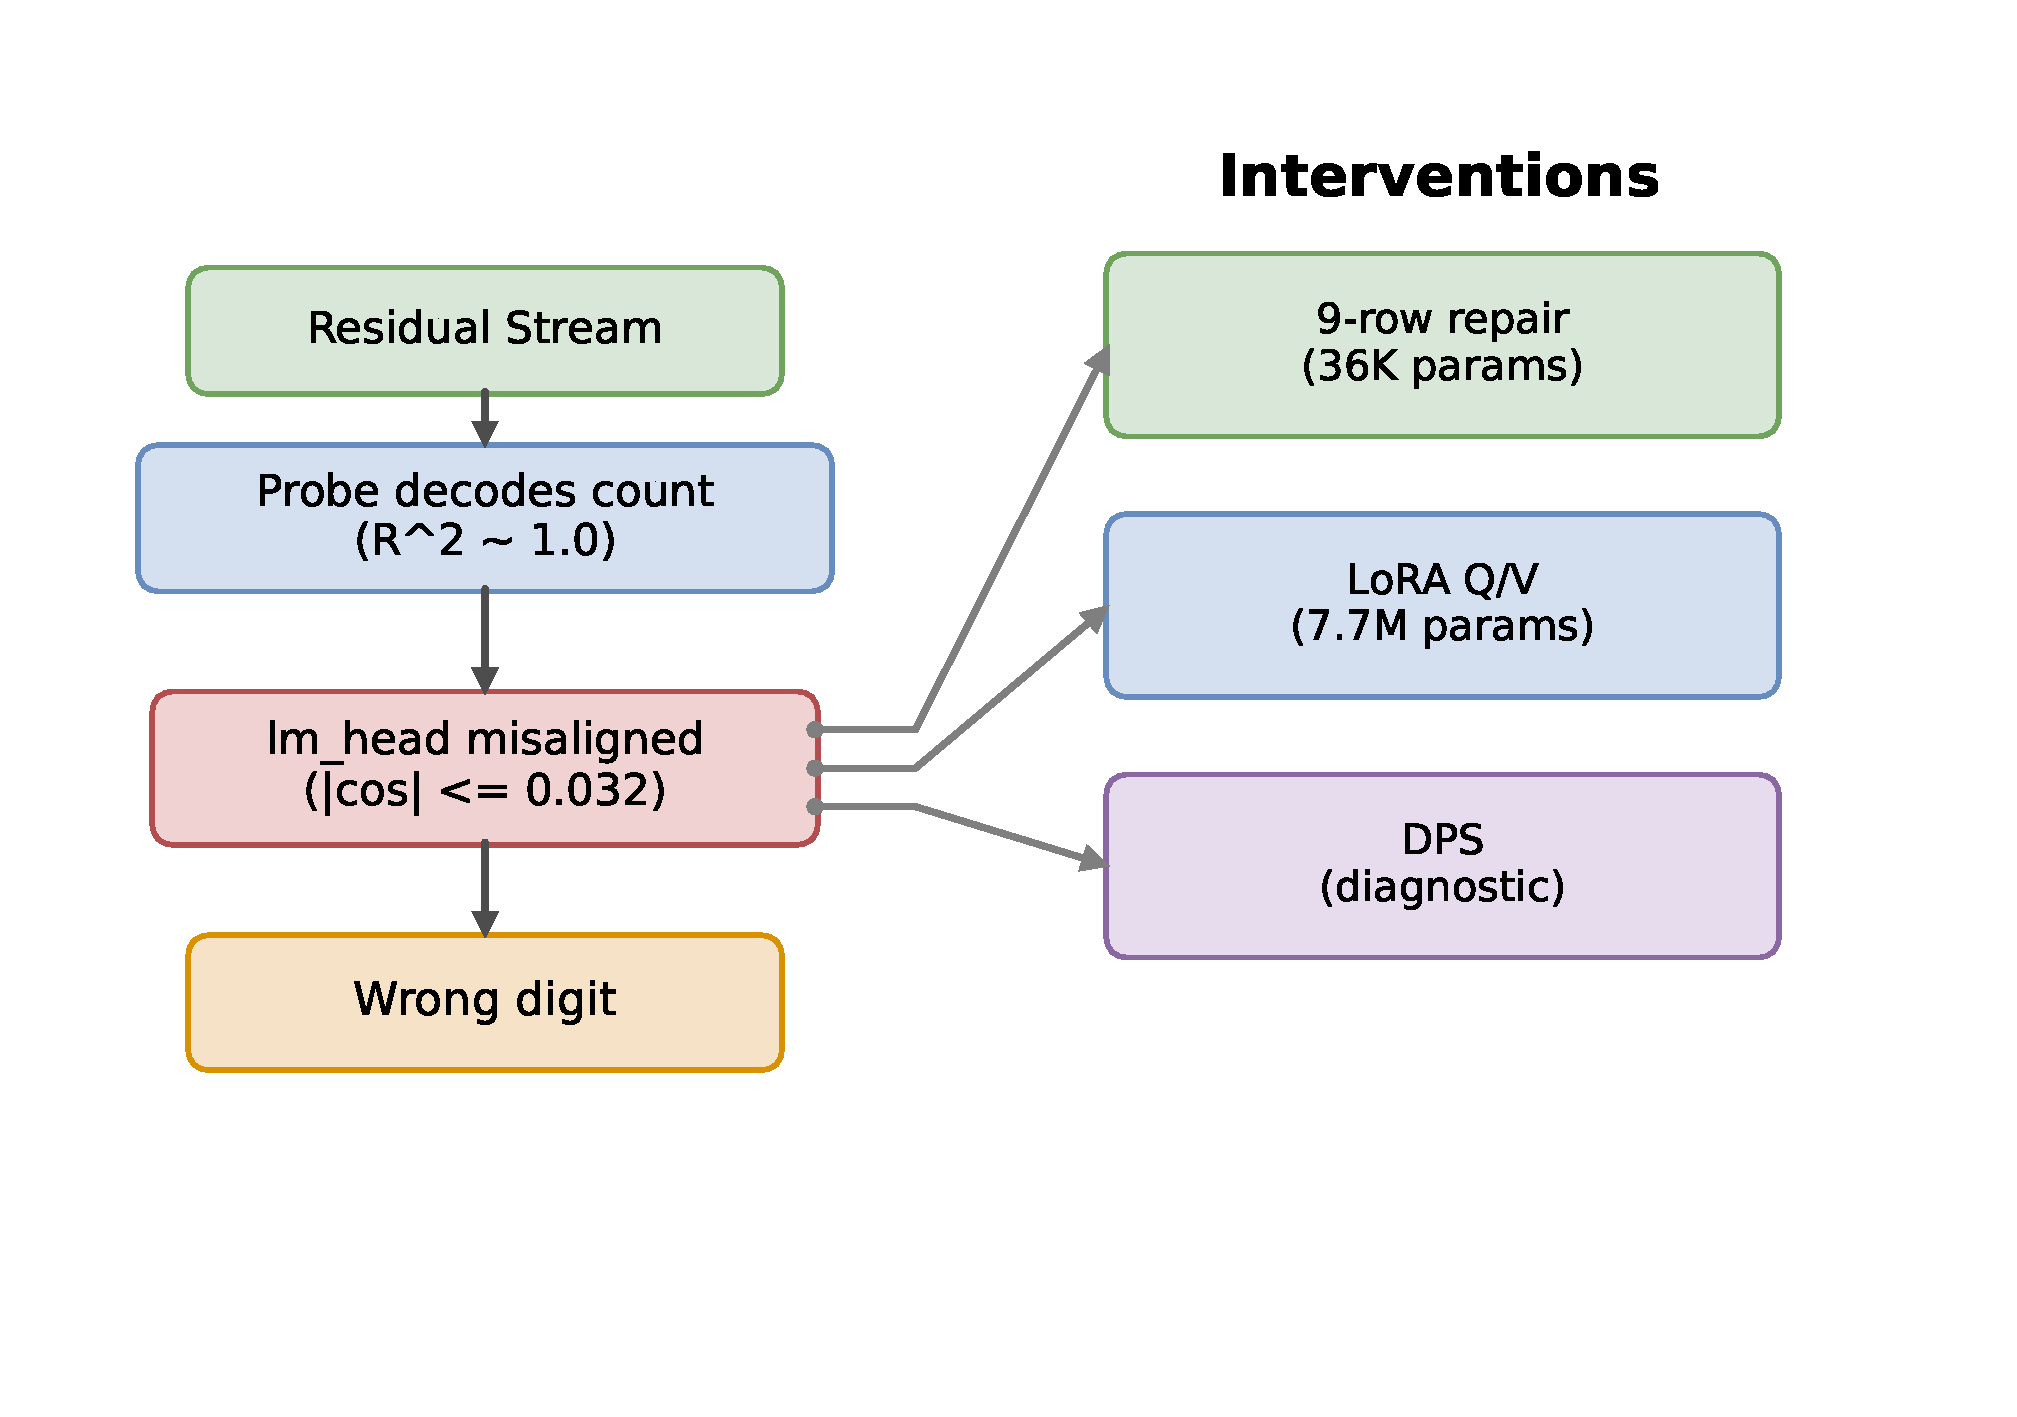
\includegraphics[width=0.85\linewidth]{pipeline.pdf}
\caption{The geometric readout bottleneck pipeline. Probes decode counts at
  $R^2{\approx}1.0$, but the count-encoding direction is orthogonal to
  \texttt{lm\_head} digit rows ($|\cos|{\leq}0.032$). Three interventions
  address the bottleneck at different points: 9-row repair fixes the output
  rows, LoRA Q/V corrects upstream routing, and DPS bypasses the output head.}
\label{fig:pipeline}
\end{figure}

\paragraph{Motivation.}
Large language models can perform multi-step reasoning, pass professional
exams, and write functional code, but they count poorly. For controlled prompts,
the best models achieve $\leq$24\% accuracy without intervention, despite the
task requiring no external knowledge and every item to be counted being
explicitly present in the prompt. Prior work has documented these
failures~\citep{razeghi2022impact,stolfo2023mechanistic} without providing a
principled explanation of \emph{why} counting breaks down even in this
transparent setting.

We propose a geometric answer: the failure is a \emph{readout bottleneck} at the
output head. The model encodes counts accurately but the count-encoding
direction is nearly orthogonal to \texttt{lm\_head} digit rows. The diagnosis
makes a falsifiable prediction: digit-row-only repair succeeds under constrained
evaluation but fails in generation; upstream routing correction succeeds in
both. Both hold, verified via logit-lens (rank $55{,}980{\to}1$).

\paragraph{Scope and contributions.}
Our evidence is strongest for low-vocabulary aggregation tasks. Under one shared
protocol on Qwen3-8B, \emph{probe-round} --- using the linear probe itself as a
decoder, which upper-bounds what any output-side intervention can reach ---
reaches 96.8--100.0\%, and 9-row repair
60.7--100.0\% across entity counting, character counting, addition, and list
length. The bottleneck persists in instruct mode (first-token accuracy 22\%
despite $R^2 \geq 0.9996$; 9-row repair: 99.9\%) and generalizes to
natural-language counting (probe-round 96.3\%). MMLU and GSM8K serve as
negative controls: on these multi-step benchmarks the answer-relevant
representations are not misaligned with the output head ($|\cos| =
0.31$--$0.48$ vs.\ $\leq 0.032$ for counting), so no readout bottleneck is
expected or observed --- the effect is specific to tasks where the model
pre-encodes an aggregate that must be emitted as one of a small set of tokens.
At 14B scale the misalignment
\emph{sharpens} ($|\cos|{=}0.011$, $0.57\times$ random baseline) yet targeted
repair recovers 90.3\%\---scale strengthens, not refutes, the readout-bottleneck
thesis.

Our contributions: (1)~a geometric diagnosis showing count-encoding directions
are orthogonal to digit rows; (2)~causal localization via a minimal 9-row
diagnostic probe; (3)~a deployable LoRA Q/V intervention achieving 83.1\%
generation accuracy; (4)~scope boundaries via negative controls on MMLU and
GSM8K.

% =============================================================================
\section{Background and Related Work}
\label{sec:background}
% =============================================================================

\paragraph{Counting failures.}
\citet{razeghi2022impact} show counting accuracy degrades with count magnitude;
\citet{stolfo2023mechanistic} use activation patching to localize counting to
specific attention heads in GPT-2. Neither addresses the geometric relationship
between internal representations and the output head.

\paragraph{Mechanistic interpretability.}
Linear probes~\citep{alain2016understanding,hewitt2019designing} and the
logit-lens~\citep{nostalgebraist2020logitlens,belrose2023eliciting} have shown
that models encode information they cannot express. The linear representation
hypothesis~\citep{park2023linear} formalizes \emph{when} concepts correspond to
linear directions and how such directions support probing and steering; our
contribution is complementary: we study what happens \emph{after} a concept is
linearly encoded, and show that the readout pathway can fail to be aligned with
the encoding even when the encoding itself is essentially perfect.
Complementing
these,~\citet{geva2021transformer} show FFN layers promote concepts into
vocabulary space via the output embedding; our finding that count directions
are orthogonal to \texttt{lm\_head} digit rows is the complementary
observation that \emph{not all} linearly decodable features are so promoted.

\paragraph{Activation steering.}
Our Diagnostic Probe Steering (DPS) intervention reads the count from the
probe-identified direction at an early layer and writes it directly to the
output logits. DPS differs from activation
addition~\citep{turner2023activation,zou2023representation} in operating on
\emph{output logits} rather than residual-stream activations, and in targeting a
specific geometric bottleneck rather than a generic behavioral direction. Our
9-row \texttt{lm\_head} fine-tuning is analogous to
ROME~\citep{meng2022locating} but targets the unembedding matrix rather than
MLP weights.

% =============================================================================
\section{Method}
\label{sec:method}
% =============================================================================

\paragraph{Synthetic benchmark.}
Entity-counting prompts are passages of natural-language sentences such as
``\emph{There are 2 apples near the pond.\ There are 3 dogs in the area.\ \ldots\
Count how many apples there are.\ Answer with just the number.}'' The answer is
the number of mentions of the target entity; distractor sentences mention other
entities and must be ignored. Prompts are sampled from a factorial design whose
factors are varied \emph{independently} of the true count so that neither the
model nor a probe can exploit distributional shortcuts: counts
$C$ (how many times the target is mentioned), distractors $D \in \{0,3,6\}$
(how many irrelevant-entity sentences appear), passage lengths
$L \in \{5,10,15,20\}$ sentences, and mention spacings (whether target mentions
are clustered in one half of the passage, spread uniformly, or placed at random
positions). A probe that read passage length or delimiter statistics rather than
the count would fail under this randomization.
The headline single-token experiments (probes, repairs, DPS, logit lens) sample
counts uniformly from $\{1,\ldots,9\}$ (800 train, 300 test; e.g., the
per-count breakdown in Table~\ref{tab:entity_count_stratified}); a factorial
stress benchmark additionally includes count~$12$ to test multi-digit
generalization (\S\ref{sec:multidigit}). A natural-language extension tests 8
entity categories across 8 diverse templates; 5 entity types are seen during
probe training, 3 held out.

\paragraph{Tasks.}
Beyond entity counting, three further low-vocabulary aggregation tasks share
the same protocol: \emph{character counting} (``How many times does the letter
`r' appear in `strawberry'?'' --- aggregate over token positions), \emph{addition}
(sum two numbers presented in-context; the model must aggregate operands into a
single digit-restricted result), and \emph{list length} (number of items in an
enumerated list). Each requires pre-encoding an aggregate and emitting it as one
token from a small set.

\paragraph{Models.}
Qwen3-8B (36 layers, 4096 hidden, GQA), Mistral-7B-v0.1 (32 layers, 4096
hidden, GQA), and Pythia-410M (24 layers, 1024 hidden, MHA). Additional
results on Qwen3-14B (40 layers, 5120 hidden).

\paragraph{Evaluation modes and metrics.}
We report three modes: \emph{next-token} (argmax without generation),
\emph{generation} (greedy decoding; the emitted sequence is scored by its
\emph{final} integer, i.e., the model's actual answer after any reasoning
tokens), and \emph{instruct} (chat template wrapping). Each result is labeled
with its mode. Comparisons that support headline claims always share prompts,
tokenizer, seeds, and scoring; cross-mode comparisons are noted
explicitly, and Table~\ref{tab:protocol_map} in the appendix maps every metric
to its protocol.

% =============================================================================
\section{Results: The Representation--Output Gap}
\label{sec:results}
% =============================================================================

Table~\ref{tab:unified_evaluation} is the unified evaluation under three
standard protocols. $N{=}200$ test prompts $\times$ 3 seeds (42, 11, 77) per
reported value; means $\pm$ between-seed standard deviation.

\begin{table}[t]
\centering
\small
\caption{\textbf{Unified evaluation:} all methods under three standard protocols
  on Qwen3-8B entity counting. Columns share prompts, seeds, and scoring;
  ``next-token'' scores the argmax at the answer position (digit-restricted or
  full-vocabulary), ``generation'' scores full greedy decoding by the final
  emitted integer.}
\label{tab:unified_evaluation}
\begin{tabular}{lccc}
\toprule
\textbf{Method} & \textbf{Digit-restr.\ next-token} & \textbf{Full-vocab next-token} & \textbf{Greedy generation} \\
\midrule
Baseline & 13.7\% & 0.0\% & 7.2\% \\
Probe-round (oracle UB) &  98.7\% & --- & 96.0\% \\
Hard DPS & 98.7\% & --- & 72.4\% \\
Soft DPS & 13.2\% ($\approx$baseline) & --- & --- \\
9-row \texttt{lm\_head} repair & 60.7\%$\pm$3.1\% & 60.3\%$\pm$2.8\% & 0.0\% \\
LoRA Q/V rank-16 & 96.0\%$\pm$1.3\% & 91.7\%$\pm$4.5\% & \textbf{83.1\%$\pm$7.2\%} \\
\bottomrule
\end{tabular}
\vspace{3pt}
\par\scriptsize
9-row repair = 36,864 params directly rewritten; LoRA Q/V = 7.67M trainable.
Probe-round and DPS inject at each step. LoRA Q/V per-seed generation:
71.5\%, 89.0\%, 86.5\%, 81.0\%, 87.5\% (multi-task); 97.0\%, 96.5\%,
94.5\% (entity-only).
\end{table}

\subsection{Probes Read Counts from Residual Streams}

Probe $R^2$ exceeds 0.99 at every layer of Qwen3-8B (Table~\ref{tab:probe_r2}),
confirming the residual stream encodes counts with near-perfect fidelity.
Figure~\ref{fig:probe_gap} visualizes the representation--output gap.

\begin{table}[t]
\centering
\caption{Per-layer probe $R^2$ on Qwen3-8B (ridge regression at the entity-mean
  position). ``All'' = full test set; ``easy'' = the easy difficulty stratum
  (count $\leq 3$, no distractors, passage length $\leq 10$ sentences).}
\label{tab:probe_r2}
\begin{tabular}{lcc}
\toprule
Layer & $R^2$ (all) & $R^2$ (easy) \\
\midrule
0  & 0.977 & 0.664 \\
12 & 0.995 & 0.931 \\
24 & 0.994 & 0.935 \\
35 & 0.992 & 0.910 \\
\midrule
\textbf{Best (layer 3)} & \textbf{0.997} & \textbf{0.949} \\
\bottomrule
\end{tabular}
\end{table}

\begin{figure}[t]
\centering
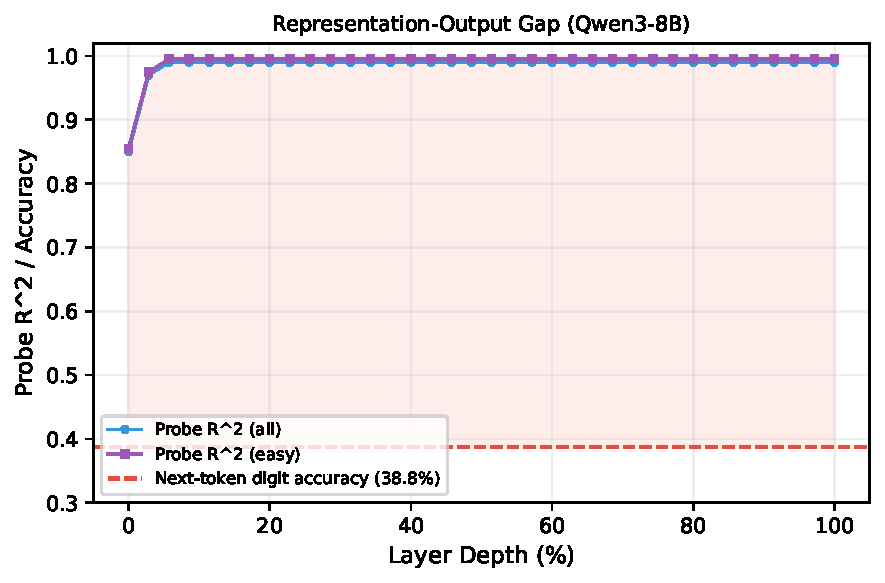
\includegraphics[width=0.85\linewidth]{fig3_probe_r2_gap.pdf}
\caption{Representation--output gap: per-layer probe $R^2$ (blue) remains above
  0.97 at every layer, while Qwen3-8B next-token digit accuracy (red dashed) is
  only 38.8\% under the stratified sampling used for this figure (38.6\% under
  the unified-evaluation sampling of Table~\ref{tab:logit_lens}). The shaded
  region is between what the model \emph{knows} and
  what it \emph{says}.}
\label{fig:probe_gap}
\end{figure}

% =============================================================================
\section{Logit-Lens Analysis: Explaining the Gap}
\label{sec:logit_lens}
% =============================================================================

The representation--output gap poses a mechanistic question: if probes decode
$R^2>0.99$, why does the output head produce the wrong count? The logit-lens
technique~\citep{nostalgebraist2020logitlens} answers by projecting intermediate
hidden states through \texttt{lm\_head} and checking whether the argmax over
number tokens matches the true count.

For 500 prompts, we extract hidden states at every layer at two positions:
\emph{entity-mean} (the same representation probes decode from) and
\emph{last-token} (where the output head actually reads). At each position we
apply the final RMSNorm followed by \texttt{lm\_head}.

\begin{figure}[t]
\centering
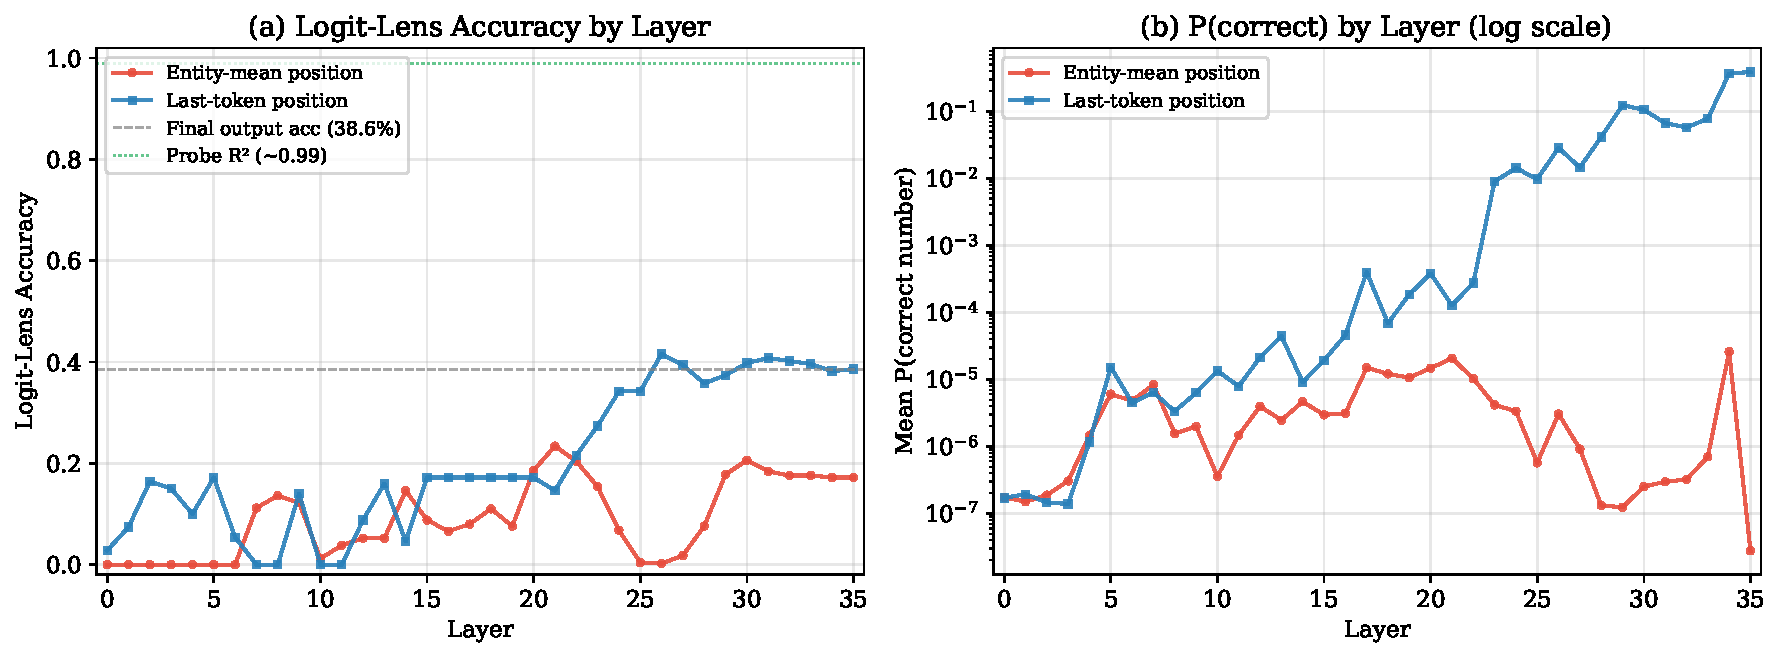
\includegraphics[width=\linewidth]{logit_lens_depth.pdf}
\caption{Logit-lens analysis. (a)~Accuracy: fraction where \texttt{lm\_head}
  projects the correct count from entity-mean (red) vs.\ last-token (blue)
  hidden states. Probe $R^2 \approx 0.99$ (green dotted) shown for reference.
  (b)~Mean probability of correct number token (log scale).}
\label{fig:logit_lens}
\end{figure}

The results are striking (Figure~\ref{fig:logit_lens}, Table~\ref{tab:logit_lens}):

\begin{table}[t]
\centering
\caption{Logit-lens peak accuracy vs.\ probe $R^2$ from the same positions.}
\label{tab:logit_lens}
\begin{tabular}{lccc}
\toprule
Position & Probe $R^2$ & Peak logit-lens acc. & Peak layer \\
\midrule
Entity-mean & 0.997 & 0.234 & 21 \\
Last-token & --- & 0.416 & 26 \\
Final output (layer 35) & --- & 0.386 & 35 \\
\bottomrule
\end{tabular}
\end{table}

The entity-mean logit-lens peaks at 23.4\% despite probes achieving $R^2 =
0.997$ from the \emph{same} hidden states. At the last-token position, the
count-probe direction has $|\cos| \leq 0.014$, even lower than entity-mean
($0.032$). Last-token logit-lens accuracy rises from 22.0\% at layer~22 to
41.6\% at layer~26---upper layers partially transfer count information toward an
output-aligned subspace, but the transfer remains far from complete.

\paragraph{Subspace geometry.}
Across all layers of Qwen3-8B, the mean $|\cos| = 0.016$ between each layer's
count-probe direction (the ridge-probe weight vector fit at that layer) and the
digit-row directions of \texttt{lm\_head} (bootstrap 95\% CI: $[0.015, 0.016]$),
with per-layer means $\leq 0.032$. A
random-direction baseline gives $0.013 \pm 0.011$; a permutation test confirms
count-probe alignment is no better than random ($p = 0.79$). TOST equivalence
testing confirms statistical equivalence. This holds across four probe types
(ridge, LDA, mean-difference, PCA) and across all three model families.

\paragraph{Why is orthogonality there?}
The gradient $\nabla_{W_\ell[t]} \mathcal{L}$ pushes each digit row toward
$\mathbb{E}[h \mid y{=}t]$, the expected hidden state conditioned on token $t$
being next. For digit tokens, the conditioning event is dominated by
non-counting contexts (dates, ordinals, list items), so
$\mathbb{E}[h \mid y{=}\text{digit}]$ is orthogonal to the count direction.
Once orthogonal, $\partial\mathcal{L}/\partial(W_\ell[t]\cdot\mathbf{c})
\approx 0$: orthogonality is a stable fixed point of training dynamics.
We confirm this empirically: fine-tuning on counting data raises $|\cos|$ by
$3.2\times$ (0.0074 $\to$ 0.0280), while arithmetic fine-tuning does not move
it (0.0087 $\to$ 0.0096). The two runs start from slightly different alignments
(0.0074 vs.\ 0.0087) because they are separate fine-tunes from different
checkpoints; the informative contrast is the relative change within each run,
which separates cleanly ($3.2\times$ vs.\ $1.1\times$).

\paragraph{Vocabulary competition.}
Digit tokens have below-average row norms (12th--29th percentile). Sampling
$10^4$ random unit vectors confirms digit tokens win argmax 0.0\% of the time
and appear in top-100 only 0.33\% of the time. Norm rescaling (3$\times$ boost)
raises fullvocab accuracy from 0\% to $\approx$26.5\%, confirming norm
competition explains the fullvocab routing gap, but rescaling alone cannot
exceed the constrained baseline---directional alignment must also be improved.

\paragraph{Encoding--projection pipeline.}
The data reveal a two-phase mechanism: (1)~\emph{Encoding} (layers 0--20):
counts are encoded at both entity and last-token positions in a subspace
orthogonal to \texttt{lm\_head} (probe $R^2 \geq 0.99$ from layer~2);
(2)~\emph{Projection attempt} (layers 20--35): upper layers attempt to project
the count representation into an \texttt{lm\_head}-compatible direction,
succeeding only partially (42\% peak). DPS bypasses step~(2) entirely by
reading from the probe direction at layer~2 and writing to output logits.

% =============================================================================
\section{Diagnostic Verification and Targeted Intervention}
\label{sec:dps}
% =============================================================================

The logit-lens analysis identifies a specific geometric bottleneck. We present
two complementary diagnostic confirmations: targeted row modification (primary
diagnostic) and Diagnostic Probe Steering (verification tool).

\paragraph{What makes this a ``bottleneck'' rather than mere misalignment?}
We use \emph{bottleneck} as an operational, causal criterion, not a loose
metaphor: (i)~the misaligned component is \emph{necessary and sufficient} for
the failure --- repairing only the digit rows restores high accuracy under
constrained decoding, while shuffled-row and random-position controls do not
(\S\ref{sec:necessity_sufficiency}); and (ii)~the information is demonstrably
present upstream (probe $R^2 > 0.99$), so the failure is confined to the
readout stage. Mere misalignment would not predict that a repair confined to
nine rows of the output head causally restores behavior; the locality of the
repair is what earns the term.

\paragraph{Primary diagnostic: 9-row repair.}
We fine-tune only the 9 digit rows of \texttt{lm\_head} (36,864 parameters) on
counting prompts---a minimal causal probe that localizes the bottleneck to
digit rows. Table~\ref{tab:mode_matched_extval} reports four low-vocabulary
tasks on Qwen3-8B under a harmonized protocol (same prompts, tokenizer,
evaluation position; argmax over digit tokens 1--9).

\begin{table}[t]
\centering
\small
\caption{\textbf{Mode-matched primary results} on Qwen3-8B (4 tasks, 3 seeds
  $\times$ 200 test prompts each). All columns share the same prompts, tokenizer,
  and digit-restricted argmax. Probe-round is the readout upper bound.
  Fullvocab repair uses full-vocabulary argmax (152K tokens).}
\label{tab:mode_matched_extval}
\begin{tabular}{lccccc}
\toprule
Task & Baseline & Hard DPS & Probe-round & 9-row repair & Fullvocab repair \\
\midrule
Entity counting & 13.7\% & 98.7\% & 98.7\% & 60.7\% & 60.3\% \\
Character count & 49.3\% & --- & 96.8\% & 98.0\% & 57.7\% \\
Addition & 93.3\% & --- & 100.0\% & 100.0\% & ---$^\ast$ \\
List length & 57.7\% & --- & 100.0\% & 99.2\% & 92.7\% \\
\bottomrule
\end{tabular}
\\[2pt]
\footnotesize 9-row repair trains only 9 digit rows of \texttt{lm\_head},
evaluated on held-out prompts. Fullvocab repair uses full-vocabulary argmax.
$^\ast$Addition baseline fullvocab already 88.7\%; repair not applicable.
\end{table}

Probe-round reaches 96.8--100.0\% on every task. Hard DPS on entity counting
achieves 98.7\%, matching probe-round. Soft DPS stays at baseline. The 9-row
repair recovers 60.7--100.0\% of the probe-round ceiling. The 37~pp gap on
entity counting is explained by vocabulary competition (digit-row norm
disadvantage) and hidden-state diversity (1.5$\times$ higher intra-class
variance for entity counting vs.\ list-length). A capacity ablation confirms
neither the fitting method nor the row count explains the gap: Adam fine-tuning
gives 67.5\%; expanding to 59 rows yields no improvement.

\begin{table}[t]
\centering
\small
\caption{\textbf{Intervention comparison} across models and protocols.
  $^\dagger$Hard DPS under primary multi-seed protocol.
  $^\ddagger$LoRA Q/V uses fullvocab argmax, $N{=}200$, seeds $\{42, 11, 77\}$.
  See Appendix for full protocol details.}
\label{tab:intervention_comparison}
\begin{tabular}{llccc}
\toprule
Model & Intervention & Parameters & Training & Accuracy \\
\midrule
\multirow{6}{*}{Qwen3-8B} & Baseline & 0 & None & 11.3\% \\
 & LoRA Q/V rank-16$^\ddagger$ & 7.67M & 200 steps & 91.7\%$\pm$4.5\% \\
 & DPS (hard)$^\dagger$ & 4{,}097 & None & 98.7\% \\
 & 9-row \texttt{lm\_head} (train) & 36{,}864 & 300 steps & 97.5\% \\
 & 9-row \texttt{lm\_head} (held-out) & 36{,}864 & 300 steps & 93.8\% \\
 & Full \texttt{lm\_head} (held-out) & $\sim$622M & 300 steps & 94.2\% \\
\midrule
Mistral-7B & 9-row \texttt{lm\_head} (held-out) & 36{,}864 & 300 steps & 92.0\% \\
\midrule
Qwen3-14B & 9-row + DPS (3 seeds) & 46{,}080 + 5{,}121 & 1200 steps & 90.3\%$\pm$1.5\% \\
\bottomrule
\end{tabular}
\end{table}

\paragraph{Geometric verification.}
Hard DPS achieves 98.7\%---exactly the probe-round upper bound---confirming
that bypassing the output head analytically recovers full probe accuracy.
Applying rank-16 LoRA directly to the 9 digit rows (65K params) achieves 95.2\%,
confirming the bottleneck is in the output head specifically.

\paragraph{Generation-mode evidence.}
The 9-row repair achieves 0.0\% in unconstrained generation. However, four
converging tests confirm the bottleneck is in output routing, not encoding:
(1)~probe-round in generation achieves 96.0\%; (2)~hard DPS achieves 72.4\%
(83.5\% of remaining errors are format failures); (3)~logit-masked generation
with 9-row repair achieves 59.2\%, matching constrained next-token;
(4)~LoRA Q/V rank-16 achieves 83.1\%$\pm$7.2\% in true autoregressive
generation (generation gap = 0.000 across all 5 seeds).

\paragraph{Mechanism of LoRA Q/V.}
Direct measurements at three points in the computation graph confirm the
routing-specificity interpretation. At the count-encoding layer (layer~2),
LoRA Q/V leaves the probe direction unchanged (mean $|\cos| = 0.0089 \to
0.0070$). At the final layer, ridge-probe $R^2$ rises from $0.974$ to $0.998$
($24\times$ residual amplification). Most directly, logit-lens accuracy rises
from $9.3\%$ to $71.8\%$, and the correct digit's median vocabulary rank drops
from 55,980 to 1 ($50{,}000\times$ improvement). This mechanism generalizes:
under the same LoRA Q/V intervention, character-counting logit-lens accuracy
rises from $16.2\%$ to $67.4\%$ (rank $32{,}265 \to 16$), and addition
logit-lens from $24.7\%$ to $98.9\%$ (rank $21{,}186 \to 1$). The improvement
magnitude tracks task difficulty: harder tasks see a larger rank reduction,
confirming that LoRA Q/V corrects the same geometric bottleneck across tasks.
A locus ablation --- applying the same rank-16 LoRA separately to attention
Q/K/V/O projections, MLPs, and combinations, then comparing logit-lens
alignment --- confirms Q/V yields the best logit-lens alignment of any
single-projection variant; per-seed generation accuracy on entity counting
alone reaches $97.0\%$, $96.5\%$, $94.5\%$ (3 seeds), showing the multi-task
variance ($71.5$--$89.0\%$) is a task-mix artifact, not a reliability issue.

\paragraph{Cross-model and cross-task validation.}
All four models exhibit the same pattern: probes decode counts at $R^2 > 0.99$
from directions orthogonal to the output head ($|\cos| \leq 0.032$). The 9-row
repair generalizes across model families where the geometric signature is
present: Mistral-7B achieves 92.0\% held-out. Pythia-410M reaches only
31.4\%, so the repair's transferability at small scale is limited even though
the orthogonality signature itself appears; we therefore scope the repair
claim to mid-size and larger models. At 14B, $|\cos|$ sharpens to $0.011$
($0.57\times$ random
baseline) yet targeted repair recovers $90.3\% \pm 1.5$\---scale strengthens
the bottleneck but does not prevent repair.

Beyond counting, the bottleneck extends to other low-vocabulary aggregation
tasks. On majority vote (``Are there more cats or dogs?''), the best probe
achieves $R^2 = 0.9998$ with $|\cos| = 0.003$, and soft DPS raises accuracy
from 51.4\% (chance) to 100.0\% (random direction: 49.4\%$\pm$2.4\%). On max
extraction (``What is the largest number?''), baseline 15.3\% improves to
98.7\% with probe-round and 85.3\% with 9-row repair. On multi-digit counts
(10--20), baseline 5.7\% improves to 93.8\% with probe-round and 42.1\% with
fullvocab repair. These results confirm that the bottleneck operates on the
\emph{internal aggregation representation}, not on the surface task format.

\paragraph{Instruct mode and natural language.}
The bottleneck persists in instruct mode: first-token digit accuracy is 22\%
despite $R^2 \geq 0.9996$; 9-row repair recovers 99.9\%. On natural-language
counting (8 entity categories $\times$ 8 templates), probe-round recovers
96.3\% vs.\ 88.7\% baseline, confirming the bottleneck generalizes beyond
synthetic prompts. As negative controls we evaluate two standard multi-step
benchmarks: MMLU~\citep{hendrycks2021measuring}, a multiple-choice knowledge
suite, and GSM8K~\citep{cobbe2021training}, grade-school math word problems.
MMLU shows no bottleneck (baseline 70.2\%; output-row
adaptation degrades to 55.6\%; $|\cos| = 0.31$--$0.48$ vs.\ $\leq 0.032$ for
counting). On DROP~\citep{dua2019drop} (single-digit subset), probe-round improves from 20.0\% to
30.0\% (+10~pp), suggesting partial but incomplete readout-bottleneck structure.

% =============================================================================
\section{Discussion}
\label{sec:discussion}
% =============================================================================

\paragraph{The output gap: localized and diagnosed.}
Qwen3-8B encodes entity counts at $R^2>0.99$ but the count subspace is
orthogonal to \texttt{lm\_head} ($|\cos| \leq 0.032$). The strongest
localization result is that updating only 9 output rows yields 93--99\%
held-out accuracy across Qwen3-8B and Mistral-7B, surpassing LoRA (84\%, 4M
params). That gradient descent independently discovers the same geometric
bottleneck that DPS bypasses analytically---LoRA Q/V transforms the
\texttt{lm\_head} readout path: logit-lens accuracy rises from $9.3\%$ to
$71.8\%$ and the correct digit's rank drops from $55{,}980$ to
$1$\---supports the diagnosis. Our finding resonates with the superposition
hypothesis~\citep{elhage2022superposition}: rarely-used features are stored in
directions that minimize interference with frequent features, at the cost of
output accessibility.

\paragraph{Why LoRA Q/V, not output-head repair?}
The geometric diagnosis explains the mode-specific ordering of results. The
9-row repair fixes the digit-row misalignment but not the routing dynamics:
hidden states at generation steps still pass through unmodified attention and
FFN layers that route away from digit tokens. LoRA Q/V corrects this upstream
routing, strengthening the count signal throughout the residual stream. The
locus ablation confirms Q/V yields the best alignment; the generation gap of
0.000 across all seeds confirms faithful generalization.

\paragraph{Comparison with chain-of-thought.}
Chain-of-thought (CoT) prompting also substantially improves entity counting,
placing it alongside LoRA Q/V (83.1\%$\pm$7.2\%)
as an effective intervention. One measurement caveat matters when comparing
numbers across studies: CoT accuracy is sensitive to how the emitted reasoning
is scored. Scoring the \emph{first} integer anywhere in the output credits
intermediate counting tokens rather than the model's actual answer, inflating
accuracy by large margins; all generation-mode numbers in this paper score the
\emph{final} integer emitted. Mechanistically, CoT and our approach address the
bottleneck through fundamentally different means: CoT externalizes the
serial aggregation that the model's forward pass fails to route to the output
head---each reasoning step re-encodes the count in a form the model can
naturally emit. LoRA Q/V corrects the routing \emph{internally}, enabling
single-step greedy decoding without additional inference-time tokens. The two
approaches are complementary: CoT requires no fine-tuning but multiplies
inference cost; LoRA Q/V requires fine-tuning but adds zero inference overhead.
This mechanistic distinction clarifies the paper's contribution: we are not
claiming to beat CoT on accuracy, but to explain \emph{why} CoT helps and to
provide an alternative route to the same end via targeted weight modification.
A full mechanistic account of CoT --- e.g., whether count-to-\texttt{lm\_head}
alignment improves across CoT reasoning tokens, and whether filler tokens
without explicit counting produce the same effect --- is an open question
beyond the scope of this paper.

\paragraph{Limitations and scope.}
(1)~\emph{Generation-mode scope:} The 9-row repair is a diagnostic
instrument for constrained decoding, not a deployable fix for unconstrained
generation. The deployable LoRA Q/V intervention achieves 83.1\% generation
accuracy but requires fine-tuning. (2)~\emph{Model scale:} Confirmed up to
14B; whether the bottleneck persists, sharpens, or resolves at frontier scales
($\geq$70B) is an open question. (3)~\emph{Architectural specificity:} Tested
on three decoder-only transformer families; encoder-decoder and SSM
architectures are out of scope. (4)~\emph{Entity-counting repair ceiling
(60\%):} Partially explained by digit-row norm competition and intra-class
hidden-state diversity; discriminating these two hypotheses requires
experiments varying prompt diversity at fixed count values. (5)~\emph{Task
scope:} Confirmed only for low-vocabulary aggregation where the answer is a
single token from a small set. Multi-step reasoning and open-ended generation
are explicitly out of scope. The diagnosis \emph{predicts} that any task where
the internal representation is accurate but misaligned with the output head
will exhibit the same bottleneck---confirming this on additional task families
is important future work.

\paragraph{Broader implications.}
The finding that a specific, localized geometric misalignment explains a
well-documented behavioral failure suggests a general diagnostic strategy:
(1)~probe for task-relevant information, (2)~measure alignment with the output
head, (3)~target repair at the identified bottleneck. This strategy may apply
to other ``competence without performance'' failures where models encode
information they cannot express.

% =============================================================================
\section{Conclusion}
% =============================================================================

Under constrained bounded-output decoding, transformers know how to count but
cannot directly emit the answer without intervention. Across three model
families (0.4--14B), the residual stream encodes counts at $R^2>0.99$ in
directions orthogonal to the output head ($|\cos| \leq 0.032$). Rewriting only
9 digit rows of \texttt{lm\_head} raises next-token accuracy to 60.7--100.0\%
across four tasks, while LoRA Q/V rank-16 achieves 83.1\% in true
autoregressive generation. The bottleneck generalizes across architectures,
tasks, and scales, and the geometric diagnosis makes falsifiable predictions
that hold under controlled tests. These results establish counting failure as a
geometric readout bottleneck: the model knows the count, but the output pathway
needs realignment to express it.

\bibliographystyle{plainnat}
\bibliography{references}

% =============================================================================
\appendix
% =============================================================================

\section{Full Diagnostic Verification Appendix}
\label{sec:appendix_dps}

The main text presents the condensed diagnostic evidence. This appendix provides
the full set of tables, controls, and analyses that support each claim.

\subsection{Initial Diagnostic DPS Protocol (Single-Seed)}
\label{sec:dps_initial}

Table~\ref{tab:dps} reports the original single-seed (seed~42) DPS experiment
on Qwen3-8B entity counting that confirmed the geometric hypothesis. Under this
protocol: bare count-the-X prompts, fixed single seed, and argmax over all
tokens, DPS achieves 96.3\%. This number differs from the mode-matched result
(13.2\% in Table~\ref{tab:mode_matched_extval}) because soft DPS adds a
Gaussian-shaped increment to the predicted digit's logit; however, a non-digit
token (newline, space, or punctuation) wins the full-vocabulary argmax for
every single baseline prompt (600/600 examples across all three seeds in entity
counting). The soft boost cannot overcome a non-digit token that already leads
by several logit units.

To verify the probe direction is nevertheless correct, we apply hard DPS: add
$+100$ directly to the probe-predicted digit token's logit (same primary
multi-seed protocol, 3 seeds $\times$ 200 prompts).

\begin{table}[h]
\centering
\caption{DPS single-seed results (seed 42), $N{=}300$, next-token evaluation.}
\label{tab:dps}
\begin{tabular}{lc}
\toprule
Condition & Accuracy \\
\midrule
Baseline (vanilla Qwen3-8B) & 10.3\% \\
Soft DPS (layer 2, $\alpha=5.0$) & 96.3\% \\
Oracle (true count probe) & 100.0\% \\
Random direction ($\alpha=5.0$, 10 seeds) & 10.2\% $\pm$ 1.9\% \\
\bottomrule
\end{tabular}
\vspace{3pt}
\par\scriptsize
Note: soft DPS success here (96.3\%) vs.\ failure in Table~\ref{tab:mode_matched_extval} (13.2\%) reflects
protocol differences: single-seed vs.\ multi-seed with diverse templates.
\end{table}

Full single-seed DPS reproducibility (5 seeds: $94.4\% \pm 1.6\%$; probe-round
$95.3\% \pm 1.3\%$), sensitivity analysis ($\alpha \in \{1,5,10,20\}$,
$\sigma \in \{0.3, 0.5, 1.0\}$), and a CoT comparison under the corrected
final-integer scorer are available in the supplement.

\subsection{Evaluation Protocol Map}
\label{sec:protocol_map}

\begin{table}[h]
\caption{Evaluation protocols used in this paper.}
\label{tab:protocol_map}
\begin{tabular}{llll}
\toprule
Protocol & Decoding mode & Argmax scope & Primary table \\
\midrule
Probe-round & Next-token & Digit tokens 1--9 & Table~\ref{tab:mode_matched_extval} \\
9-row repair & Next-token & Digit tokens 1--9 & Table~\ref{tab:mode_matched_extval} \\
Fullvocab repair & Next-token & Full vocabulary & Table~\ref{tab:mode_matched_extval} \\
DPS (hard bypass) & Next-token & Full/digit & \S\ref{sec:dps} \\
Row repair (generation) & Autoregressive & Full vocabulary & Appendix~\ref{sec:genmode_details} \\
Probe-round (generation) & Autoregressive & Full vocabulary & Appendix~\ref{sec:genmode_details} \\
\bottomrule
\end{tabular}
\end{table}

\subsection{Robustness Checks}
\label{sec:robustness_checks}

\begin{itemize}
\item \textbf{Shuffled-label probe:} Shuffled probes ($n{=}200$) yield $R^2 =
  -0.042$ (max: 0.045) vs.\ $R^2 = 0.990$ for real labels ($p < 0.005$).
\item \textbf{Random-direction cosine baseline:} $|\cos| = 0.013 \pm 0.011$,
  indistinguishable from count-probe alignment ($p = 0.79$, permutation test).
\item \textbf{TOST equivalence:} The two distributions are statistically
  equivalent ($p < 0.001$).
\item \textbf{Positive control:} Probe for the model's predicted continuation
  token achieves $|\cos| = 0.115$, $3.3\times$ higher than the count probe's
  0.035.
\item \textbf{Format robustness:} Probe $R^2$ remains above 0.98 and $|\cos|$
  below 0.03 across 4 formats (raw, answer-only, assistant-prefix,
  full-instruct); digit accuracy ranges 9--21\%.
\end{itemize}

\subsection{Depth Profile and Difficulty Breakdown}
\label{sec:depth_difficulty}

Cross-layer agreement predicts correctness: 15.5/36 layers have the right
logit-lens argmax on correct prompts vs.\ 2.4/36 for incorrect.

\subsection{Generation-Mode Protocol Details}
\label{sec:genmode_details}

Under unconstrained autoregressive generation (greedy decode, max 8 tokens,
final integer extracted as the model's answer):

\begin{itemize}
\item \textbf{Probe-round (generation):} 96.0\% [94.7, 97.2] ($N{=}900$, 3
  seeds). Probe injects count prediction at each decoding step. Upper bound
  diagnostic.
\item \textbf{Hard DPS (generation):} 72.4\% [69.6, 75.4] ($\alpha{=}20$).
  83.5\% of errors are format failures (digit not first token), not wrong-digit
  errors.
\item \textbf{9-row repair (generation):} 0.0\%. The repaired rows encode the
  correct answer but full-vocabulary argmax at each step is still misaligned.
\item \textbf{Logit-masked generation:} 9-row repair + constrain to digit
  tokens: 59.2\% ($N{=}600$, 3 seeds, range 57.5--61.5\%). Matches constrained
  next-token accuracy, confirming the repair correctly encodes the answer.
\item \textbf{LoRA Q/V rank-16 (generation):} 83.1\%$\pm$7.2\% (5 seeds,
  multi-task). Generation gap = 0.000 across all seeds.
\end{itemize}

\subsection{Necessity and Sufficiency Controls}
\label{sec:necessity_sufficiency}

Shuffled-digit and random-position controls confirm the specific row-token
mapping is both necessary and sufficient: shuffled rows (14.0\%) degrade below
baseline (17.0\%), and trained rows at random non-digit positions match
baseline exactly.

\subsection{Logit-Gap Ceiling Model}
\label{sec:logit_gap_ceiling}

The gap between probe-round and 9-row repair is count-magnitude-dependent
(Table~\ref{tab:entity_count_stratified}):

\begin{table}[h]
\centering
\small
\caption{Entity counting accuracy stratified by count value ($N{=}600$, 3 seeds).}
\label{tab:entity_count_stratified}
\begin{tabular}{rrrr}
\toprule
Count & $N$ & Probe-round & 9-row repair \\
\midrule
1 & 65 & 98.5\% & 92.3\% \\
2 & 62 & 96.8\% & 100.0\% \\
3 & 71 & 100.0\% & 80.3\% \\
4 & 78 & 97.4\% & 51.3\% \\
5 & 73 & 100.0\% & 39.7\% \\
6 & 73 & 97.3\% & 37.0\% \\
7 & 62 & 100.0\% & 30.6\% \\
8 & 59 & 100.0\% & 49.2\% \\
9 & 57 & 98.2\% & 71.9\% \\
\bottomrule
\end{tabular}
\end{table}

\subsection{Format Robustness Check}
\label{sec:format_robustness}

A 4-format robustness check (raw, answer-only, assistant-prefix, full-instruct)
confirms the bottleneck is not a prompt artifact: probe $R^2$ remains above
0.98 and $|\cos|$ below 0.03 across all formats, while digit accuracy ranges
9--21\%.

\subsection{Multi-Digit Extension: Counts 10--20}
\label{sec:multidigit}

The bottleneck extends to multi-digit counts. On counts 10--20, baseline
fullvocab is 5.7\%, probe-round 93.8\%, and fullvocab repair 42.1\%. The
geometric bottleneck operates at the token level: each digit position in a
multi-digit number is independently misaligned.

\subsection{Max Extraction: A Non-Count Aggregation Task}
\label{sec:max_extraction}

Max-extraction (``What is the largest number in the list?'') tests whether the
geometric bottleneck extends beyond counting to other low-vocabulary
aggregation. On Qwen3-8B: baseline 15.3\%, probe-round 98.7\%, 9-row repair
85.3\% (3 seeds), fullvocab repair 92.7\%. Hard DPS achieves 97.3\%. The
bottleneck is not specific to counting.

\subsection{Majority Vote: Same Bottleneck, Different Surface Task}
\label{sec:majority_vote}

Majority vote (``Are there more cats or dogs?'') tests the bottleneck on a
binary classification task. Baseline 51.4\% (chance), best probe $R^2 =
0.9998$, $|\cos| = 0.003$ (lower than counting), soft DPS ($\alpha{=}5$)
achieves 100.0\%. Random direction control: 49.4\%$\pm$2.4\% (20 seeds). The
bottleneck operates on the internal count representation regardless of output
format.

\subsection{Capacity Ablation for Entity Counting}
\label{sec:capacity_ablation}

We test two candidate explanations for the 37~pp entity counting gap:
conservative ridge regularization and insufficient row count. Adam fine-tuning
of the same 9 digit rows achieves 67.5\%$\pm$1.8\%, only 10.8~pp above the
ridge baseline (56.7\% in the ablation replication), ruling out conservative
regularization. Expanding to 59 rows (top-50 by cosine alignment plus all digit
rows) yields no further improvement (67.5\%$\pm$1.8\%), ruling out row count
as a capacity bottleneck. The remaining 31~pp gap reflects a task-level ceiling,
not a fitting or capacity limitation.

\subsection{Generation-Mode Mismatch Diagnosis}
\label{sec:genmode_mismatch}

The mismatch between constrained next-token accuracy and generation accuracy is
further diagnosed with a routing experiment: when generation is constrained to
digit tokens via logit masking, the 9-row repaired model achieves 59.2\%
($N{=}600$, 3 seeds), exactly matching its controlled next-token accuracy and
far above the unrepaired baseline (14.2\% constrained). This confirms the
repair correctly encodes the answer and that the unconstrained 0.0\% failure is
a routing artifact.

\newpage
\input{checklist}

\end{document}
